\documentclass
[	10pt, 			% размер шрифта
	aspectratio=43	% соотношение сторон слайдов
]{beamer}	

\usetheme[]{metropolis}				% тема презентации
\usefonttheme[]{professionalfonts}  % запрещаем beamer'у перезаписывать мат. шрифты

%% Пакеты и их настройки
\usepackage[]{fontspec}         % загрузка шрифтов, работа с кодировкой и пр.
\usepackage[]{polyglossia}      % переносы слов
\usepackage[]{microtype}        % различные исправления типографии
\usepackage[]{unicode-math}     % использование математических символов юникода

\usepackage[]{graphicx}
\usepackage[]{subfig}
\usepackage[]{float}
\usepackage[]{enumitem}
\usepackage[]{tabularx}
\usepackage[]{booktabs}

\frenchspacing                  %% убираем лишние отступы после точек

%% Перенос слов
\binoppenalty       = 10000 %% Запрет переносов строк в формулах
\relpenalty         = 10000
\pretolerance       = 5000  %% Настройки переноса
\tolerance          = 9000  %% Настройки переноса
\emergencystretch   = 0pt   %% Запрещаем выход за границы
\righthyphenmin     = 2     %% целое число, равное наименьшему количеству букв в слове, которые можно переносить на следующую строку
\lefthyphenmin      = 2
\hyphenpenalty      = 500
\clubpenalty        = 10000 %% Запрет разрывов страниц после первой
\widowpenalty       = 10000 %% и перед предпоследней строкой абзаца

%% Язык
\setmainlanguage[spelling=modern]{russian}
\setotherlanguage{english}

%% Шрифты
\defaultfontfeatures{Ligatures  = {TeX, Common},
	Mapping    = tex-text}

%% Main font
\setmainfont
[   Path            = ../fonts/,
	Extension       = .otf,
	UprightFont     = *-Regular,
	BoldFont        = *-Bold,
	ItalicFont      = *-Italic,
	BoldItalicFont  = *-BoldItalic
]{FreeSerif}
\newfontfamily\cyrillicfont
[   Path            = ../fonts/,
	Extension       = .otf,
	UprightFont     = *-Regular,
	BoldFont        = *-Bold,
	ItalicFont      = *-Italic,
	BoldItalicFont  = *-BoldItalic
]{FreeSerif}

%% Roman font
\setromanfont
[   Path            = ../fonts/,
	Extension       = .otf,
	UprightFont     = *-Regular,
	BoldFont        = *-Bold,
	ItalicFont      = *-Italic,
	BoldItalicFont  = *-BoldItalic
]{FreeSerif}
\newfontfamily\cyrillicfontrm
[   Path            = ../fonts/,
	Extension       = .otf,
	UprightFont     = *-Regular,
	BoldFont        = *-Bold,
	ItalicFont      = *-Italic,
	BoldItalicFont  = *-BoldItalic
]{FreeSerif}

%% Sans font
\setsansfont
[   Path            = ../fonts/,
	Extension       = .otf,
	UprightFont     = *-Regular,
	BoldFont        = *-Bold,
	ItalicFont      = *-Oblique,
	BoldItalicFont  = *-BoldOblique
]{FreeSans}
\newfontfamily\cyrillicfontsf
[   Path            = ../fonts/,
	Extension       = .otf,
	UprightFont     = *-Regular,
	BoldFont        = *-Bold,
	ItalicFont      = *-Oblique,
	BoldItalicFont  = *-BoldOblique
]{FreeSans}

%% Mono font
\setmonofont
[   Path            = ../fonts/,
	Extension       = .otf,
	UprightFont     = *-Regular,
	BoldFont        = *-Bold,
	ItalicFont      = *-Oblique,
	BoldItalicFont  = *-BoldOblique
]{FreeMono}
\newfontfamily\cyrillicfonttt
[   Path            = ../fonts/,
	Extension       = .otf,
	UprightFont     = *-Regular,
	BoldFont        = *-Bold,
	ItalicFont      = *-Oblique,
	BoldItalicFont  = *-BoldOblique
]{FreeMono}

%% Math font
\setmathfont
[   Path        = ../fonts/,
	Extension   = .otf,
	BoldFont    = *Bold
]{XITS-Math}


%% ---------------------------------------------------------------------
%% Настройки пользователя
%% ---------------------------------------------------------------------

\graphicspath{{images/}}
\metroset{numbering   = fraction,
	      progressbar = frametitle,
	      background  = light}

\title{Тема презентации}
%\subtitle{Южный Федеральный Университет\\ Институт ММиКН им. Воровича}
\author{Студент 4 курса \\ А.\,А. Иванов \\\vskip 1mm Научный руководитель: \\ д.\,ф.-м.\,н., профессор В.\,С. Пилиди \vskip 1em}
%\institute{Институт ММиКН им. Воровича}
\date{30 февраля 2020 г.}


\begin{document}
	\maketitle
	% !TEX root = ../presentation.tex

\begin{frame}{Постановка задачи}
$\bullet$ Задача 1

$\bullet$ Задача 2

$\bullet$ Задача 3
\end{frame}
	% !TEX root = ../presentation.tex

\begin{frame}{Задача 1}
	Фильтр минимизирует срендеквадратическое отклонение цвета пикселя.
	
	\begin{equation*}\label{eq:wiener_nsr}
	\hat{Y}(i, j) = \left[ \frac{\hat{H}^*(i, j)}{\left|\hat{H}(i, j)\right|^2 + \frac{S_n(i, j)}{S_s(i, j)}} \right] \times \hat{F}(i, j),
	\end{equation*}
где
\begin{itemize}[noitemsep]
	\item $Y$ -- восстановленное изображение,
	\item $F$ -- наблюдаемое изображение,
	\item $H$ -- функция рассеивания,
	\item $H^*$ --комплексное сопряжение $H$,  
	\item $S_n$ -- энергетический спектр шума -- $\left| \hat{N} \right|^2$,
	\item $S_s$ -- энергетический спектр исходного изображения -- $\left| \hat{F} \right|^2$,
	\item $\times$ -- умножение комплексных чисел.
\end{itemize}
\end{frame}
	% !TEX root = ../presentation.tex

\begin{frame}{Слайд 3. Изображения}
\begin{figure}[H]
	\captionsetup[subfigure]{justification=centering, labelformat=empty}
	\subfloat[Наблюдаемое изображение]{
\includegraphics[width=0.4\textwidth]{wiener_blurred}}%
	\quad
	\subfloat[Восстановленное изображение]{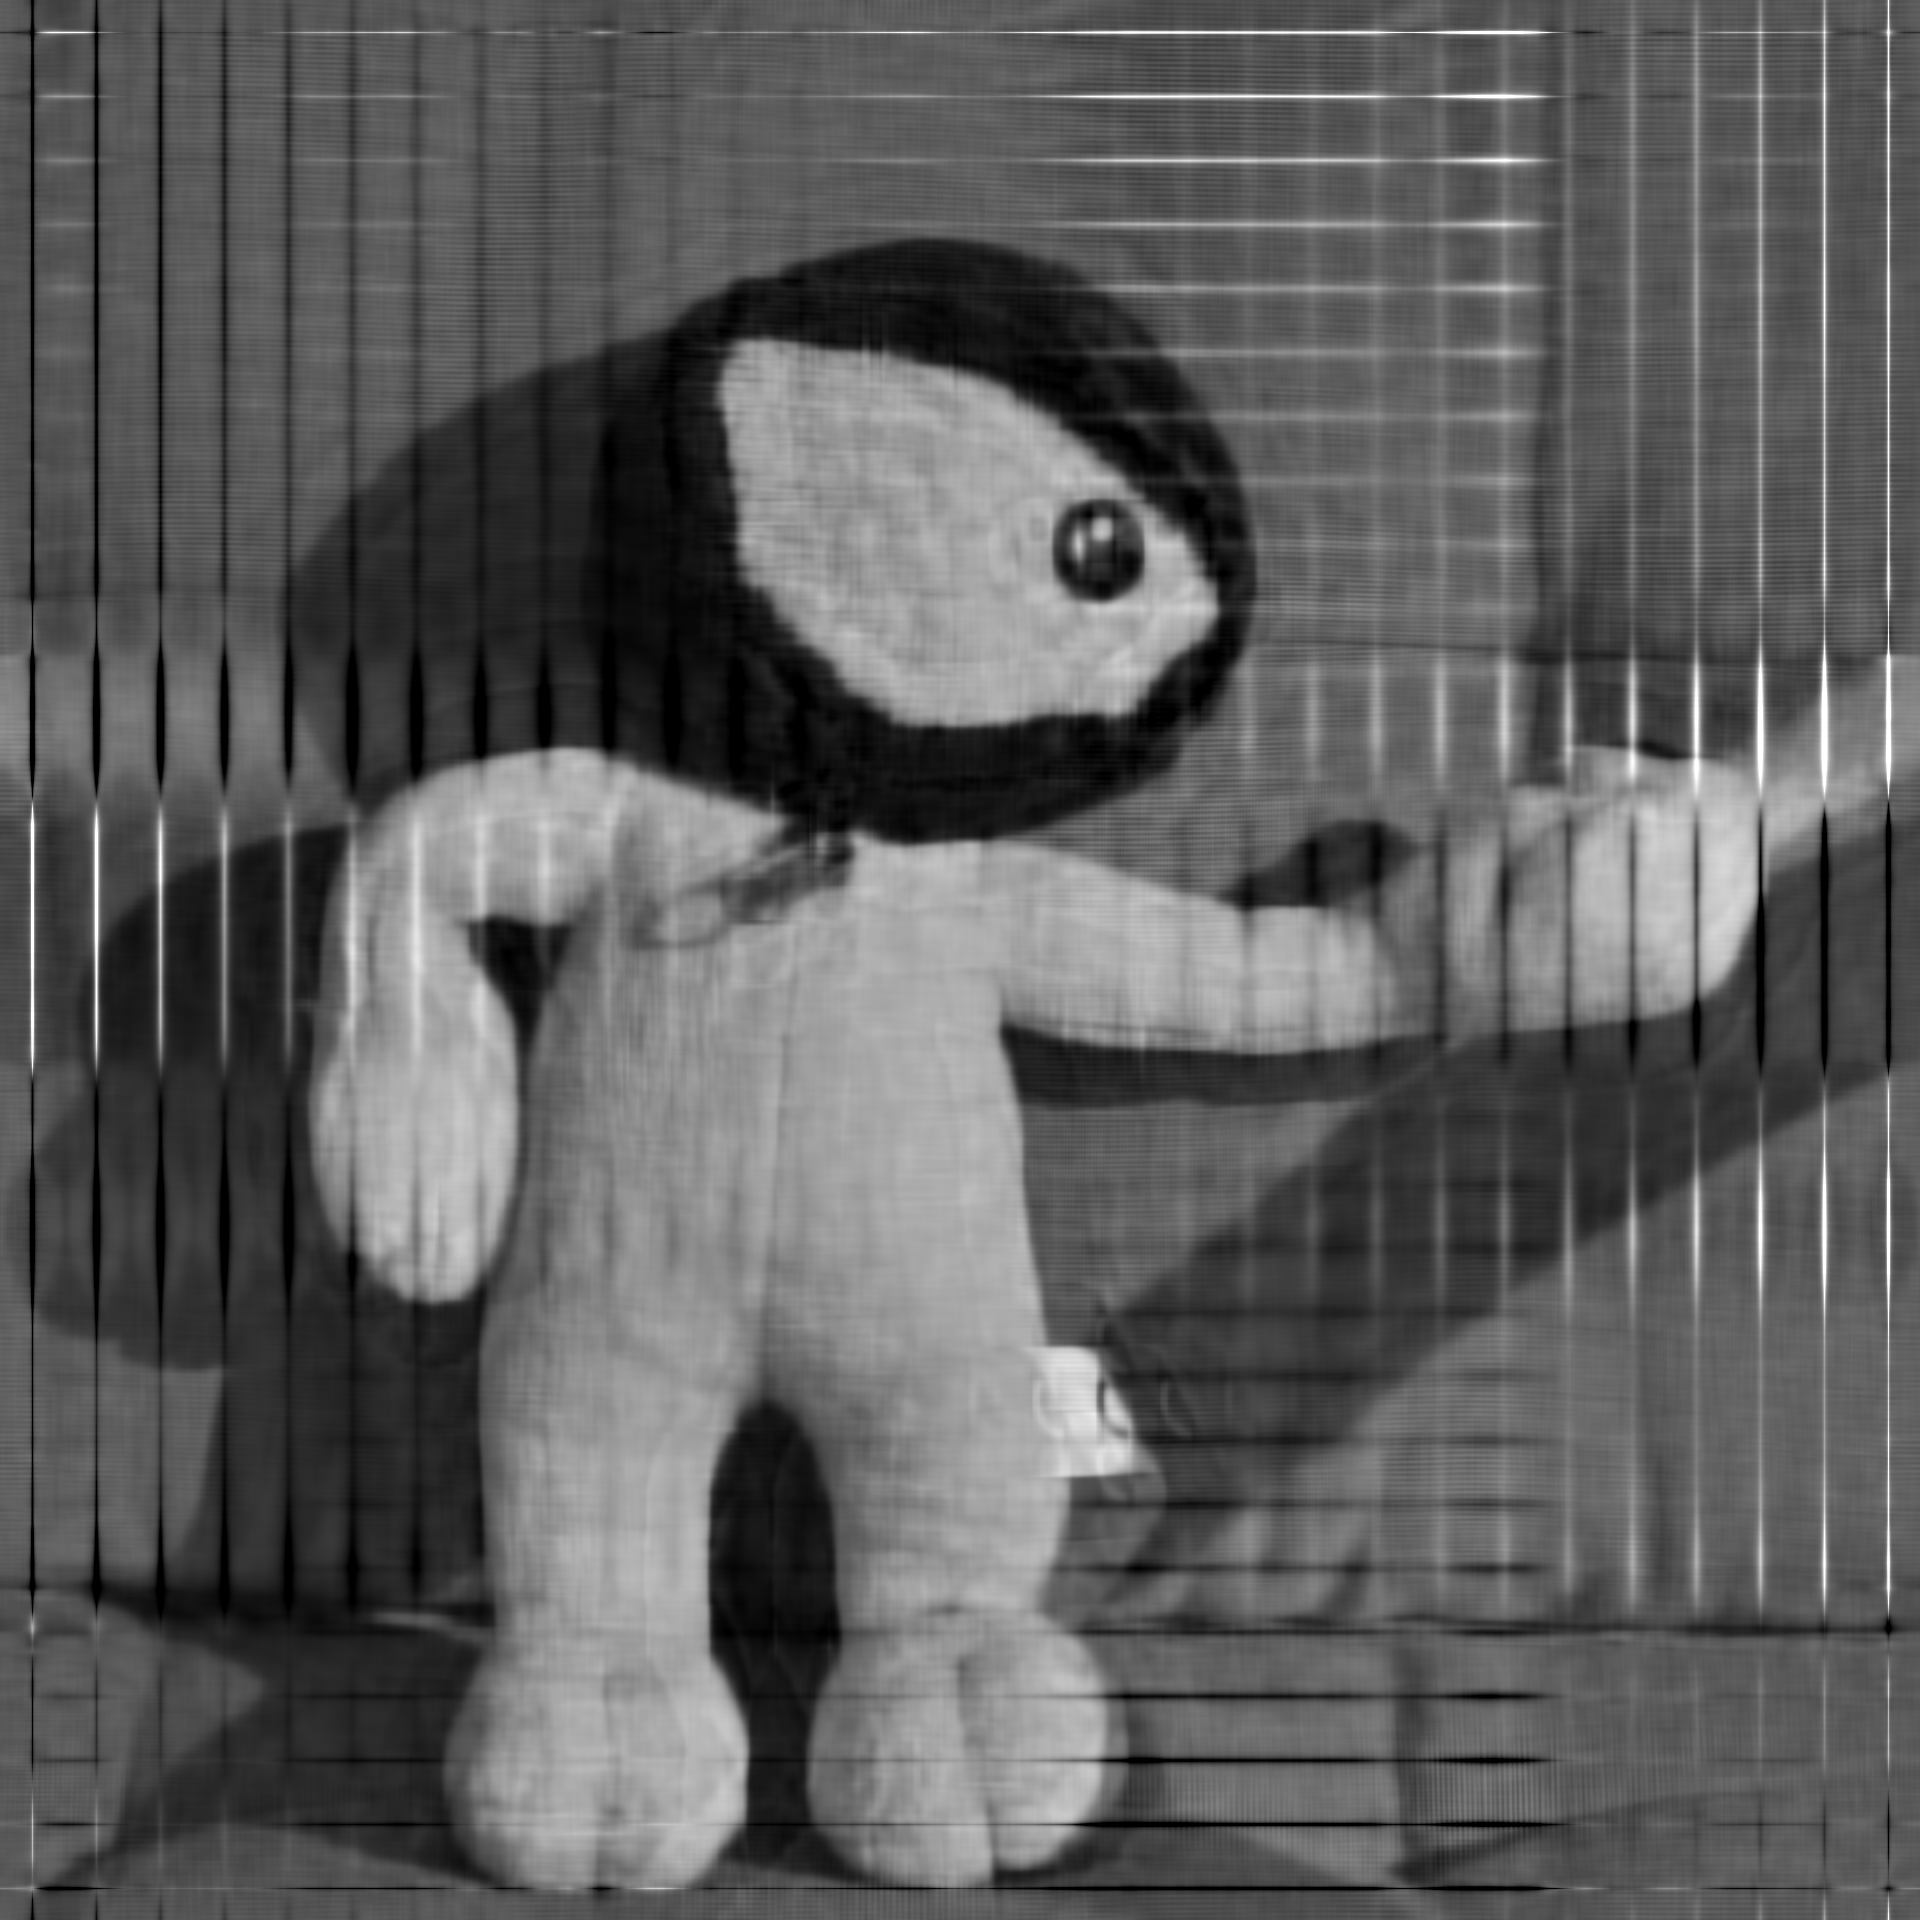
\includegraphics[height=0.4\textwidth]{wiener_nsr_nonzero}}%
\end{figure}
	
\end{frame}
	% !TEX root = ../presentation.tex

\begin{frame}{Слайд 4}
Описание слайда
    \begin{table}[H]
    \centering
    \caption{\label{tab:widgets}Подпись к таблице --- сверху}
        \begin{tabular}{llr}
            \toprule
                  \multicolumn{2}{c}{Item}        &           \\
            \cmidrule(r){1-2}
        Животное & Описание & Цена (\$) \\ \midrule
            Armadillo                  & frozen   &      8.99 \\ \bottomrule
        \end{tabular}
    \end{table}
\end{frame}
	\begin{frame}{Результаты работы}
$\bullet$ Результат 1

$\bullet$ Результат 2

$\bullet$ Результат 3

\end{frame}	
\end{document}